%%%%%%%%%%%%%%%%%%%%%%%%%%%%%%%%%%%%%%%%%%%%%%%%%%%%%%%%%%%%%%%%%%%%%%%%%%%%%%%%
\documentclass[twocolumn]{revtex4}

% Include some extra packages.
\usepackage[]{graphicx}
%%%%%%%%%%%%%%%%%%%%%%%%%%%%%%%%%%%%%%%%%%%%%%%%%%%%%%%%%%%%%%%%%%%%%%%%%%%%%%%%
\begin{document}

%%%%%%%%%%%%%%%%%%%%%%%%%%%%%%%%%%%%%%%%%%%%%%%%%%%%%%%%%%%%%%%%%%%%%%%%%%%%%%%%
\title{
Predicting The Weather
}

\author{Mike Adamski}
\affiliation{Siena College, Loudonville, NY}

\date{\today}

\begin{abstract}
    The main procedure was to apply heavy usage of the \begin{it} Monte Carlo \end{it} technique to several scenarios and assumptions about the weather in order to determine things like: did it rain? If so, how much? Monte Carlo method essentially allows me to generate hundreds of thousands of sample "months" in only a few seconds to make generalizations about the likelihood of a certain event happening. I have run specific tests using this and have determined: 
\begin{itemize} %creates bulleted list
	\item That there is approximately a .93\% of rain on one and only one day in the month, assuming a 20\% chance of rain.
    \item That there is approximately a .77\% of rain on eight or more days that month, assuming a 10\% chance of rain. 
    \item Based upon a series of assumptions which indicate a more typical chance of rain, along with assumptions for the amount of rain for a certain area, I expect around a 34\% chance of getting 10cm or more of rain in a month.
    \item Based on these same events in the prior bullet, the average rainfall per month was approximately 8.65cm.
    \item Most importantly, from my findings I determined that I am 95\% confident that the rainfall will be between 0 and 21cm.
\end{itemize}

\end{abstract}

\maketitle

\section{Introduction}
%%%%%%%%%%%%%%%%%%%%%%%%%%%%%%%%%%%%%%%%%%%%%%%%%%%%%%%%%%%%%%%%%%%%%%%%%%%%%%%%
	The rational behind this project was to utilize coding along side statistical probability in order to effectively "predict the weather," more specifically precipitation. I was trying to find out if by analyzing trends and using predetermined assumptions, I could go as far as to create a 95\% confidence interval in regards to expected range for rainfall in any given month, using strictly statistics and Python. In simple terms, the overall objective of the project was to see how accurately I could predict weather based upon huge randomly generated samples. 

%%%%%%%%%%%%%%%%%%%%%%%%%%%%%%%%%%%%%%%%%%%%%%%%%%%%%%%%%%%%%%%%%%%%%%%%%%%%%%%%
\section{Problem One}
The goal of this problem was to determine the probability of it raining one and only one day in a month, assuming a 20\% chance of rain on any particular day.

I accomplished this by first importing NumPy, a useful tool for any numerical calculations. Next, I initialize two instance variables, one is the numbers of months to be simulated, the other stores the number of occurrences. After this, I loop through all the previously defined number of months. Each iteration I reset a counter variable for the number of days rained to zero. Then, I create an array of 30 random numbers between one to five. This represents the assignment of a number, each with a 20\% chance of occurring, to a day of the month. After, within this loop, I create another loop to go through each day in the month. In this sub-loop, there is a conditional to check if my 20\% case has occurred, if so, I add one to my rain counter. Outside of the individual day sub-loop, there is a conditional to check if the number of days rained in the previous 30 day loop is exactly equal to one (only one day rained in the month), if this is the case, I increment my number of occurrences by one. Finally, I print out the number of total occurrences in the total number of months tested. Then directly after, I print the percent of the event occurring.
\begin{it}Results can be seen in the abstract.
\end{it}
%%%%%%%%%%%%%%%%%%%%%%%%%%%%%%%%%%%%%%%%%%%%%%%%%%%%%%%%%%%%%%%%%%%%%%%%%%%%%%%%
\section{Problem Two}
The goal of problem two is to determine the probability that it rains at least eight days in a month, assuming only a 10\% chance of rain each day. Problem two is nearly identical to problem one in terms of code the only changes to the procedure can be seen in bold below:\newline


"I initialize two instance variables, one is the numbers of months to be simulated, the other stores the number of occurrences. After this, I loop through all the previously defined number of months. Each iteration I reset a counter variable for the number of days rained to zero. Then, I create an array of 30 random numbers between \begin{bf}one to ten.\end{bf} This represents the assignment of a number, each with a \begin{bf}10\% chance of occurring\end{bf}, to a day of the month. After, within this loop, I create another loop to go through each day in the month. In this sub-loop, there is a conditional to check if my 20\% case has occurred, if so, I add one to my rain counter. Outside of the individual day sub-loop, there is a conditional to check if the number of days rained in the previous 30 day loop is\begin{bf} greater than or equal to eight (rained eight or more days that month)\end{bf}, if this is the case, I increment my number of occurrences by one. Finally, I print out the number of total occurrences in the total number of months tested. Then directly after, I print the percent of the event occurring."\newline

\begin{it}Results can be seen in the abstract.
\end{it}
%%%%%%%%%%%%%%%%%%%%%%%%%%%%%%%%%%%%%%%%%%%%%%%%%%%%%%%%%%%%%%%%%%%%%%%%%%%%%%%%
\section{Problem Three}
This problem has multiple assumptions, the first of which are in regards to whether or not it rained on a particular day. These are as follows:
\begin{itemize} %creates a list
    \item If it is the first day of the month, there is a 10\% chance of rain.
    \item If it rained 1 day before, but not 2 days before, there is a 20\% chance of rain.
    \item If it rained both of the 2 days before, but not the 3rd day before, there is a 25\% chance of rain.
	\item If it rained for the 3 days (or more) before, there is a 5\% chance of rain.
    \item Otherwise, there is a 10\% chance of rain
\end{itemize}
The other set of assumptions relates to, if it rained, how much it rained that day in terms of centimeters. These are as follows:
\begin{itemize} %creates a list
    \item 1 cm 20\% 
    \item 2 cm 30\%
    \item 3 cm 30\%
    \item 4 cm 10\%
    \item 5 cm 10\%
\end{itemize}
The goal of the problem is based on both these sets of facts, what is the probability that it will rain at least 10cm in a given month?

In order to better grasp the many moving parts in problem three, I will break the problem into sub-parts.
\subsection{Instance Variables}
I start off by initializing and defining several variables which will be used later on in this problem. I have one which simulates the number of months which will be tested which is set to a sample size of 100,000. The next is a two are simple counter variables set to zero, one which will be used later to increment by one each time my conditional of 10cm of rain in the month has been met, the other to count total number of months tested (slightly redundant but makes the code more understandable). Lastly, I initialized an empty array which will later have our monthly rain totals appended to it. 

\subsection{CmRained Function}
This function accepts one parameter, which will be an integer for the number of days it rained later on in the problem.It starts by initializing a local variable to zero which will be used to sum the total rain for the given number of days. The function will then loop through the number of days passed in each time doing the following:

It creates a new array of random numbers from one to ten (each number has a 10\% probability of occurring). Next the loop checks a conditional which corresponds to two numbers totaling a 20\% chance of occurrence, if either of which are hit, so to speak, then this adds one centimeter of rain to my previously defined sum variable. Next, if the two numbers are not hit, a similar process occurs except with three more unused numbers, which symbolizes a 30\% chance of occurrence If hit, it adds two centimeters of rain to my sum variable. If not, it moves on to the next conditional which checks another three unused numbers of the ten possibilities (30\% chance). If hit, three centimeters are added to the sum variable. In the case it is not, the next conditional is checked. If one of the two remaining unused variables is hit (10\% chance), then four centimeters are added to the sum variable. Otherwise, if none of the previous numbers hit, there is only one remaining number(remaining 10\% chance), which will cause the loop to add 5cm to sum variable. As previously stated this is all within the loop.

Outside the loop, there is one simple return, which yields the total sum variable which has been being increased through each iteration. 

\subsection{"Master Loop"}
The master loop essentially will execute the bulk of the code for problem three. It will start with a loop, which will iterate through the number of months I wish to simulate. Within this loop we have the following:
Two counter variables are defined and reset to zero each iteration. Next we have code to handle the first day of the month test case. While this is redundant since both the first day and a "normal" day with not previous days of rain have a 10\% chance of rain, it helps to conceptually to break out the separate case as it is listed in the initial bullet. To handle this first day case, I set a variable equal to a random number between one and ten (10\% chance per number). If a conditional looking for only one number of the ten potential numbers is hit, the counts for both number of days rained and for the number of previous days is incremented by one (signaling it rained).

Next, I create an array of 29 random numbers (not 30 because we already handled the first day of the month) between one and 20, each with a 5\% chance of occurring. After this, I created a loop which will loop 29 times through a series of conditionals. The first conditional checks it rained the prior day, if so, it hits another conditional which uses the random number array sub-iteration number to create a 20\% range. If the number falls within this range, both number of days rained and number of days rained previously are incremented by one. If not, number of days of previous rain is reset to zero (symbolizing that it did not rain that day). The next outer conditional checks if it rained the two prior days consecutively. If so the inner conditional uses the random number array again to simulate a 25\% chance range. If the number is within the range, both number of days rained and number of days rained previously are incremented by one. If it is out of the range, it means it did not rain that day and I reset the previous day count to zero once again. The third outer conditional checks if the number of previous consecutive days of rain is greater than or equal to three. If so, the inner conditional uses the random number array to simulate a 5\% occurrence chance. If the number is hit, then both number of days rained and number of days rained previously are incremented by one. If the number is not hit, number of previous consecutive days is reset again to zero. The last outer statement hits only if all the other previous conditionals have not hit (meaning there have been no consecutive days of rain at that particular day). If this happens then an inner conditional using my random numbers searches for two specific numbers out of the 20 generated, which simulates a 10\% chance. If one of the two numbers hits, then both number of days rained and number of days rained previously are incremented by one. Should the number not hit, number of previous consecutive days of rain is set to zero (it did not rain). Finally the inner loop is finished at this point. However, within the main loop for each month, I now want to use my previously created CmRained. I use a conditional to check if when the number of days it rained in the month, when passed to my CmRained function, is greater or equal to ten. If this is the case I increment both my counter instance variables I previously defined in the prior subsection by one, one indicates that the test passed and the other just keeps a count for total tests. If the prior conditional is false, I only increment the counter for total tests by one. Finally the last thing in the master loop, is a statement to append the amount of rain in centimeters for the month to my previously empty array.

\subsection{Final Calculation}
I now set my counter variables for number of tests passed and total tests to type float to ensure accurate division in the next step. I create a new variable which is set to:
$$\frac{PassedTests}{TotalTests} * 100 $$ %creates a centered fraction

This represents the probability that I can expect to see 10 or more centimeters of rain in a given month. Finally, I print this out within a string to display my result in a more understandable way.

\begin{it}Results can be seen in the abstract.
\end{it}
%%%%%%%%%%%%%%%%%%%%%%%%%%%%%%%%%%%%%%%%%%%%%%%%%%%%%%%%%%%%%%%%%%%%%%%%%%%%%%%%
\section{Problem 3B}
The objective of this problem is to make a visual distribution of my expected rainfall values for each month. This will be done by creating a histogram containing all the prior Monte Carlo trials.

First, I define the size of my (to be created) figure setting it to five by five. Next, I plot my data values which are found in the array containing the samples of monthly rain from problem three. These values are placed within 30 bins (one bin for every centimeter of rain displayed),which span from zero to to 30, which is where nearly all the rainfall measures fall. Next I create labels for both the x and y axis, where x is the amount of rainfall and y is the number of occurrences from the total sample. Following this, I create a basic title for the graph. Lastly I set the layout to tight, this makes sure the graph fits in the plot area which I defined. The outcome of this can be seen in Figure~\ref{rain} below.

\begin{figure}[h] %placed here "h"
\centering
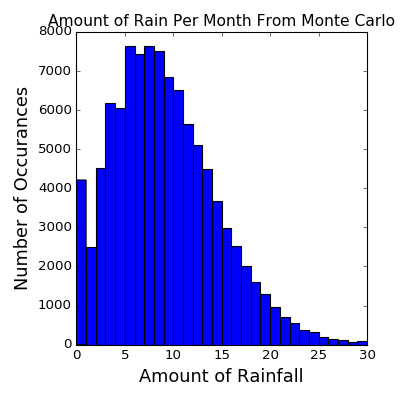
\includegraphics[width=0.40\textwidth]{monte_carlo_graph_mike_adamski.png}
\caption{Visual distribution of rainfall values.\label{rain}}
\end{figure}
%%%%%%%%%%%%%%%%%%%%%%%%%%%%%%%%%%%%%%%%%%%%%%%%%%%%%%%%%%%%%%%%%%%%%%%%%%%%%%%%
\section{Problem 3C}
The goal for this sub-problem is to find the average amount of rainfall that can be expected from any given month.

I start by initializing a variable to zero, that will keep track of a sum throughout this problem. Next, I create a loop that will go through the entire length of all my previously created Monte Carlo trials. Each iteration of the loop it will simply add that months rain precipitation total to my sum variable. After the loop is finished I then create another variable and assign it the value of my total divided by the total number of months, thus giving an average rainfall per month. This result is then printed to the screen within a simple string. 

\begin{it}Results can be seen in the abstract.
\end{it}

%%%%%%%%%%%%%%%%%%%%%%%%%%%%%%%%%%%%%%%%%%%%%%%%%%%%%%%%%%%%%%%%%%%%%%%%%%%%%%%%
\section{Problem 3D}
The goal of this problem is to be able to create an accurate 95\% confidence interval to present a range of the expected rainfall amounts. This is done by eliminating the top and bottom 2.5\% of values from our sorted array to find the "edges," which we can use in our range. 

To go about this I first created a copy of my Monte Carlo trials array (assigned it to another array), that way any changes made within this problem to the entries in the array will not effect any other problems and will not prevent me from re-running the problem multiple times (which would eliminate the top and bottom 2.5\% every time. I then sort the data in my new array using the built in python sort function which sorts the values in ascending order. I then create a variable and assign it to 2.5\% of the length of my total trial array and set it to type integer so I am able to use it within my splicing. I then set my array copy to that same array but starting at the index position of my 2.5\% variable I just created, this effectively eliminates the bottom 2.5\% of values. Next, I similarly set my array copy to the same array but have my upper bound stop at the total length reduces by my 2.5\% variable, thus eliminating the top 2.5\% of values in my array. 

After I am down to the middle 95\% of data values, I can now assume that the first spot and the last spot are my "edges" to be used within my confidence interval (index location zero and index location at the position one before total length). I assign both values to two separate variables to use in print statements. I use several print statements which display the resulting range and where the numbers are from in the array. 

\begin{it}Results can be seen in the abstract.
\end{it}

%%%%%%%%%%%%%%%%%%%%%%%%%%%%%%%%%%%%%%%%%%%%%%%%%%%%%%%%%%%%%%%%%%%%%%%%%%%%%%%%
\end{document}

